\documentclass{article}

\usepackage[dvipsnames]{xcolor}
\usepackage{corl_2026}

\usepackage{graphicx}
\usepackage{amsmath,amssymb}
\usepackage{booktabs}
\usepackage{enumitem}
\usepackage{subcaption}


\title{Does Auxiliary Spatial Supervision Make Vision-Language-Action Models Safer?\\ A Factorial Analysis}

\author{
Anonymous Author(s)
}

\begin{document}
\maketitle

\begin{abstract}
Fine-tuned Vision-Language-Action (VLA) models achieve high task success yet remain collision-prone. We ask whether auxiliary spatial supervision during fine-tuning can improve collision avoidance, and conduct a systematic $2{\times}2$ factorial study crossing gradient flow with normalization type, supplemented by ablations of label content, reference frame, and temporal extent (twelve conditions in total). The answer depends critically on \emph{how} the auxiliary head is attached. The best configuration, detached gradients with LayerNorm, reliably outperforms the no-auxiliary baseline, raising Collision Avoidance Rate from $0.745$ to $0.802$ with a large effect size. The naive default, BatchNorm with full gradient flow, is associated with reduced safety relative to baseline. A factorial analysis disentangles two additive factors: gradient flow through BatchNorm reduces safety, possibly mediated by running-statistics corruption during auxiliary forward passes; LayerNorm, which normalizes per-token without shared batch statistics, provides a consistent safety advantage regardless of gradient flow. Surprisingly, the spatial content of the labels (ground-truth occupancy, random noise, or depth) has no detectable effect under the original codebase; the gradient pathway, not spatial information, appears to determine the outcome. These safety effects are invisible to standard task-success benchmarks (TSR ANOVA all $p{>}0.27$), explaining why fifteen prior spatial VLA methods did not detect them. The auxiliary head is discarded at inference, adding zero deployment cost.
\end{abstract}

\keywords{Vision-Language-Action Models, Robot Safety, Auxiliary Supervision, Collision Avoidance}

\section{Introduction}

Vision-language-action (VLA) models achieve high task success on manipulation benchmarks~\cite{brohan2023rt2, kim2024openvla, kim2025oft}, but behavioral safety does not follow. On SafeLIBERO Level~I~\cite{hu2025vlsa}, OpenVLA-7B reaches 87.8\% Task Success Rate but only 74.5\% Collision Avoidance Rate (CAR), with per-task collision rates reaching 43--93\% on the three most constrained tasks (Appendix, Table~\ref{tab:per_task}).

Two active research threads address related but distinct aspects. The first enriches VLAs with auxiliary spatial prediction (occupancy grids, depth maps, point clouds)~\cite{li2026spatialforcing, yuan2025depthvla, wu2025spatialvla, liu2025occvla}. At least fifteen such methods have appeared in the past year~\cite{wu2026stvla, chen2026gstvla, tu2026sgvla, xiao2026stemvla, li2025pointvla, sun2025geovla, bhat20253dcavla, li2025qdepthvla, abouzeid2025geoaware, rao2026augvla3d, li2026corridorvla}, all reporting improved task success under the implicit assumption that spatial awareness yields safer behavior. The second targets VLA safety directly through runtime action filtering~\cite{hu2025vlsa, zhai2026cofreevla, raja2024ogmcbf} or constrained RL~\cite{zhang2025safevla}. These lines are disconnected: no spatial method evaluates collision avoidance, and no safety method examines spatial representations. A recent survey~\cite{li2026vlasafety} confirms this gap. Moreover, single-factor ablations, the dominant methodology, cannot decompose joint effects of multiple design choices; only a factorial design can determine whether factors like gradient flow and normalization type interact or combine independently.

\begin{figure*}[t]
\centering
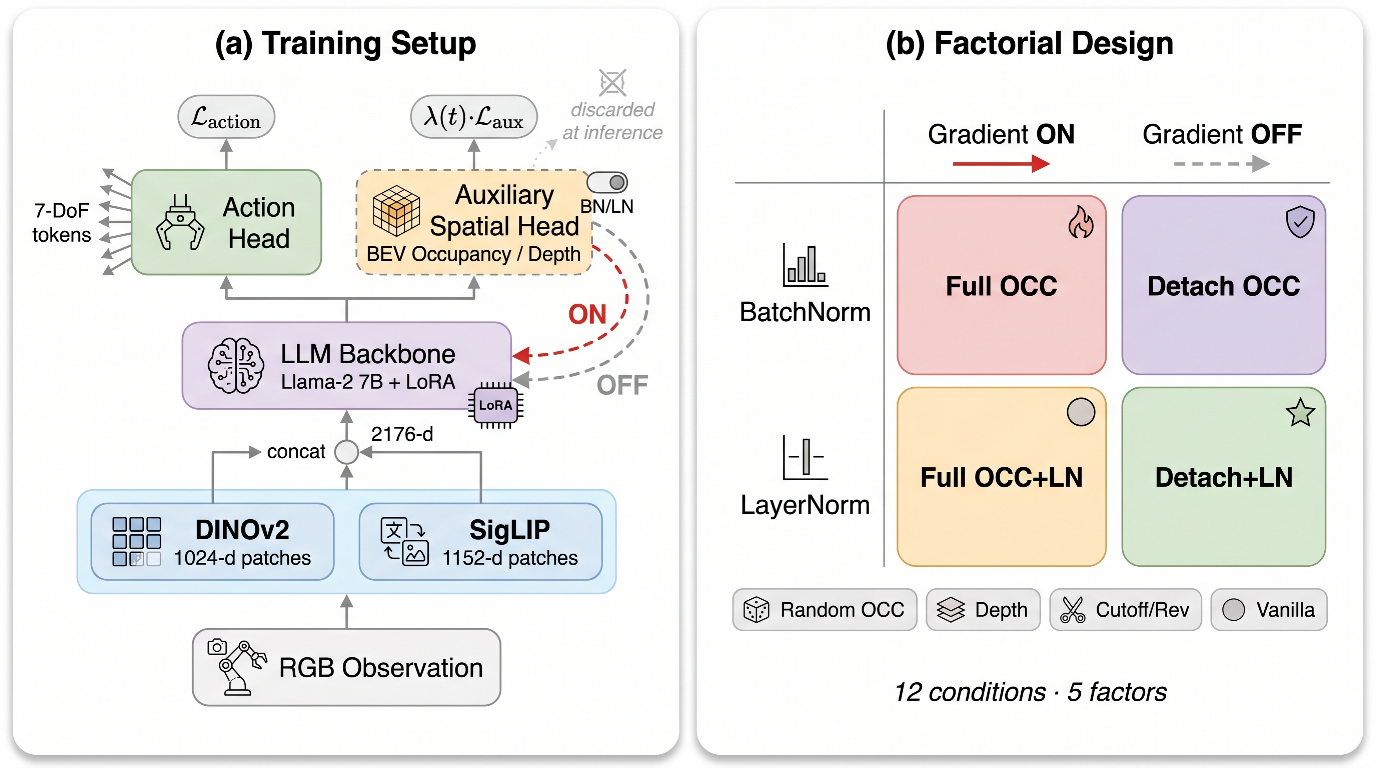
\includegraphics[width=\textwidth]{figures/fig1_architecture_pb.pdf}
\caption{\textbf{Training setup and factorial design.} \textbf{(a)}~OpenVLA-7B with dual vision encoders (DINOv2 + SigLIP) and an auxiliary spatial head (bird's-eye view occupancy or depth), discarded at inference. \textbf{(b)}~$2{\times}2$ factorial crossing gradient flow (ON/OFF) and normalization (BN/LN), plus Vanilla baseline and 7 single-factor ablations probing label content, reference frame, and temporal extent.}
\label{fig:overview}
\end{figure*}

% fig:results_bar moved into fig:car_factorial (a)

We ask a direct question: does auxiliary spatial supervision during VLA fine-tuning improve collision avoidance? We conduct a systematic factorial study using OpenVLA-7B~\cite{kim2024openvla} with LoRA~\cite{hu2022lora}. A core $2{\times}2$ factorial crosses gradient flow (ON/OFF) with normalization (BN/LN); seven additional single-factor ablations probe label content, spatial reference frame, and temporal extent, twelve conditions in total (Figure~\ref{fig:overview}). The factorial design can detect interactions that single-factor studies miss; here, it establishes that the two main effects are additive (\S\ref{sec:results}), a practically important finding that prior work could not have obtained.

The central finding is that \textbf{Detach+LN consistently outperforms Vanilla}, raising CAR from $0.745$ to $0.802$ with a large effect size. The factorial design reveals why: gradient flow through BatchNorm degrades safety, while LayerNorm provides a consistent advantage, and these two effects combine additively. Only the BN + gradient flow combination falls below Vanilla. Spatial label content showed no detectable effect under the v1 codebase (\S\ref{sec:results}).

Our contributions:
\begin{enumerate}[nosep,leftmargin=*]
    \item \textbf{Two additive factors govern safety, not spatial content.} Detached gradients with LayerNorm yield the highest collision avoidance rate, reliably outperforming the no-auxiliary baseline with a large effect size. A $2{\times}2$ factorial identifies two additive factors: gradient flow through BatchNorm degrades safety; LayerNorm provides a consistent protective effect. These safety effects are invisible to standard task-success benchmarks (TSR ANOVA all $p{>}0.27$), explaining why fifteen prior methods did not detect them. Spatial label content shows no detectable influence under the original codebase (Table~\ref{tab:main_results}, Figure~\ref{fig:car_factorial}b), with the normalization advantage amplifying fourfold on physically constrained tasks where safety margins are thinnest.

    \item \textbf{Factorial methodology for VLA auxiliary heads.} The first systematic factorial comparison of how auxiliary head design choices combine during VLA fine-tuning. The factorial design establishes that effects are additive, a conclusion single-factor ablations cannot reach (\S\ref{sec:ablation}, Table~\ref{tab:ablation_design}).

    \item \textbf{Actionable guidelines at zero cost.} Do not add auxiliary spatial heads with gradient flow under BN. If required, use detached gradients with LayerNorm. BN + gradient flow additionally exhibits $5$--$7{\times}$ cross-seed variance, making safety outcomes unpredictable across training runs. No ground-truth spatial labels are needed; the auxiliary head is discarded at inference (\S\ref{sec:discussion}).

    \item \textbf{Codebase sensitivity as a confound.} Implementation details dominate safety signals: a single code revision shifts CAR by up to 8.6\,pp, exceeding the largest experimental effect (${\leq}5.7$\,pp), questioning the reproducibility of safety claims across existing spatial VLA methods (\S\ref{sec:discussion}, Appendix~\ref{app:codebase}).
\end{enumerate}


\section{Related Work}

\subsection{VLA Safety and Spatial Representations}

Generalist VLAs~\cite{black2024pi0, team2024octo} and existing safety approaches~\cite{hu2025vlsa, zhai2026cofreevla, raja2024ogmcbf, zhang2025safevla} do not examine whether spatial representations contribute to safety. A parallel line enriches VLAs with 3D structure (depth fusion, representation alignment, geometric encoding, or occupancy prediction)~\cite{yuan2025depthvla, li2025qdepthvla, rao2026augvla3d, bhat20253dcavla, abouzeid2025geoaware, yang2024depthanything, li2026spatialforcing, wu2025spatialvla, li2025pointvla, sun2025geovla, wu2026stvla, chen2026gstvla, tu2026sgvla, xiao2026stemvla, li2026corridorvla, liu2025occvla, li2022bevformer, sima2023occnet, tian2023occ3d}, yet none evaluates collision avoidance. Occupancy prediction originated in autonomous driving~\cite{li2022bevformer, sima2023occnet, tian2023occ3d}; OccVLA~\cite{liu2025occvla} adapted it to robotic VLAs. SpatialVLA~\cite{wu2025spatialvla}, DepthVLA~\cite{yuan2025depthvla}, and OccVLA report task success improvements but no safety metrics. The assumption that spatial awareness should improve safety remains untested; we address this gap.

\subsection{Auxiliary Tasks and Multi-Task Gradient Dynamics}

Multi-task learning exploits shared representations~\cite{caruana1997multitask, ruder2017overview}, with approaches ranging from universal representations~\cite{bilen2017universal} and task-dependent attention~\cite{maninis2019astmt} to residual adapters~\cite{rebuffi2018adapters}. However, auxiliary tasks risk negative transfer through optimization conflict or generalization failure~\cite{chen2018gradnorm, yu2020pcgrad, liu2021cagrad, navon2022nashmtl, jiang2023forkmerge}. PCGrad~\cite{yu2020pcgrad} and CAGrad~\cite{liu2021cagrad} assume gradient conflict as the primary failure mode; our analysis shows near-zero action--auxiliary cosine similarity, which points to a different mechanism.

BatchNorm~\cite{ioffe2015batchnorm} couples representations to batch statistics; its sensitivity to minibatch composition~\cite{ioffe2017renorm} and covariate shift~\cite{schneider2020bn, li2017adabn} becomes consequential when auxiliary tasks alter training distributions. LayerNorm~\cite{ba2016layernorm} computes per-token statistics independently. For VLA fine-tuning with LoRA~\cite{hu2022lora}, the interaction between auxiliary losses and low-rank adapter updates has not been studied; our factorial design isolates gradient flow from spatial content.



\section{Method}

We fine-tune OpenVLA-7B~\cite{kim2024openvla} with the OFT recipe~\cite{kim2025oft}, which concatenates DINOv2~\cite{oquab2024dinov2} (1024-d) and SigLIP~\cite{zhai2023siglip} (1152-d) patch features into a 2176-dimensional representation per spatial token. We apply LoRA~\cite{hu2022lora} (rank 32, $\alpha{=}16$) and augment the action prediction loss with an auxiliary spatial prediction head:
\begin{equation}
\mathcal{L}_\text{total} = \mathcal{L}_\text{action} + \lambda(t) \cdot \mathcal{L}_\text{aux}(h(\phi_v(o_t)), s_t^*),
\quad \lambda(t) = 0.01 \cdot \exp(-t / 50000)
\end{equation}
where $h$ denotes the auxiliary head, $\phi_v$ the frozen-then-LoRA-adapted vision encoders, and $s_t^*$ the ground-truth spatial label at step $t$. The coefficient $\lambda(t)$ decays exponentially so that spatial gradients shape early representations without dominating late-stage action refinement. The auxiliary head is discarded at inference, incurring zero additional cost.

\textbf{Bird's-eye view (BEV) occupancy head.} The head (1.2M parameters) maps the 256 patch tokens from the current observation frame to a $64{\times}64$ binary occupancy grid. A linear projection ($2176{\to}256$) is reshaped to $16{\times}16$, followed by two transposed convolutions ($256{\to}128{\to}64$, kernel 4, stride 2) each with BatchNorm2d and GELU, and a final $1{\times}1$ convolution with sigmoid activation. Ground-truth grids are rendered from MuJoCo simulator state replay by projecting object bounding boxes onto the table-plane BEV. Training uses focal loss~\cite{lin2017focal} ($\alpha{=}0.25$, $\gamma{=}2.0$) to handle class imbalance in the sparse occupancy signal. The initial auxiliary weight $\lambda_0{=}0.01$ is set to keep auxiliary gradients below 2\% of the action loss magnitude, avoiding interference with action learning.

\textbf{Monocular depth head.} This head shares the BEV architecture but uses ReLU/smooth-L1 on $64{\times}64$ egocentric depth maps from MuJoCo, complementing the allocentric BEV grid.

\subsection{Ablation Design}
\label{sec:ablation}

We evaluate twelve conditions organized around a $2{\times}2$ factorial core crossing gradient flow (ON/OFF) with normalization (BN/LN), supplemented by single-factor ablations along three additional dimensions (Table~\ref{tab:ablation_design}). The factorial core comprises: \textbf{Vanilla} (no auxiliary head), \textbf{Full OCC} (BEV occupancy, gradient flow, BN), \textbf{Detach OCC} (gradients blocked via \texttt{stop\_gradient}), and their LN variants (\textbf{Full OCC+LN}, \textbf{Detach+LN}). Seven supplementary conditions probe label content (\textbf{Random OCC}), reference frame (\textbf{Depth}), and temporal extent (\textbf{Cutoff@\{15K--45K\}}, \textbf{Reverse Cutoff}; Appendix~\ref{app:training}).

Formally, let $\text{sg}(\cdot)$ denote the stop-gradient operator. Full conditions compute $\mathcal{L}_\text{aux}(h(\phi_v(o_t)), s_t^*)$, so auxiliary gradients flow through $\phi_v$. Detach conditions compute $\mathcal{L}_\text{aux}(h(\text{sg}(\phi_v(o_t))), s_t^*)$: the head trains on encoder features but no gradient reaches $\phi_v$. This separates bidirectional coupling (spatial and action objectives jointly shape representations) from unidirectional readout.

\begin{table}[t]
\centering
\small
\setlength{\tabcolsep}{4pt}
\caption{Ablation design: each comparison isolates one factor.}
\label{tab:ablation_design}
\begin{tabular}{@{}ll@{}}
\toprule
Comparison & Isolated Factor \\
\midrule
Full OCC vs.\ Vanilla & Auxiliary spatial supervision \\
Random vs.\ Full OCC & Spatial content vs.\ gradient flow \\
Detach vs.\ Vanilla & Encoder gradient flow (presence/absence) \\
Detach+LN vs.\ Detach OCC & Normalization (BN vs.\ LN) without gradient flow \\
Full OCC+LN vs.\ Full OCC & Normalization (BN vs.\ LN) with gradient flow \\
$2{\times}2$ factorial & Normalization $\times$ gradient flow combined effects \\
Depth vs.\ Full OCC & Egocentric vs.\ allocentric frame \\
Cutoff@\{15K--45K\} vs.\ Full OCC & Temporal extent of gradient flow \\
Reverse Cutoff vs.\ Cutoff@35K & Early vs.\ late gradient flow \\
\bottomrule
\end{tabular}
\end{table}

\subsection{Evaluation}

We evaluate on SafeLIBERO Level~I~\cite{hu2025vlsa}, which places obstacles in close proximity to manipulation targets across 10 tabletop tasks drawn from LIBERO-Spatial~\cite{liu2023libero}. We report two metrics: \textbf{Task Success Rate (TSR)}, the fraction of completed episodes, and \textbf{Collision Avoidance Rate (CAR)}, where a collision is registered when the L1 displacement of any obstacle exceeds $10^{-3}$. Core factorial conditions use 3--4 independent seeds; supplementary conditions use 1--3 seeds (Table~\ref{tab:main_results}); each seed runs 50 rollouts per task (500 episodes per seed).

The BN and LN factorial cells have been trained under a revised codebase (v2, 3--4 seeds each) that fixed a batch-index resume bug present in v1; both versions share identical architectures, hyperparameters, and evaluation protocols, but the bug fix shifts absolute CAR by up to 8.6\,pp for auxiliary conditions (Section~\ref{sec:discussion}). Supplementary conditions use the original codebase (v1). Training runs for 50K steps on a single NVIDIA RTX PRO 6000 GPU; full details are in Appendix~\ref{app:training}.



\section{Results}
\label{sec:results}

\subsection{Main Results}

Table~\ref{tab:main_results} summarizes TSR and CAR across conditions (50 rollouts $\times$ 10 tasks per seed). $\Delta$CAR is computed against the matched-codebase Vanilla baseline (v2: $0.745 \pm 0.024$, 3 seeds, for factorial conditions above the midrule; v1: 0.780 for supplementary conditions below). Random OCC ($^\star$) uses v1 code but is included above the midrule as a factorial control; its $\Delta$CAR is omitted due to the cross-codebase baseline mismatch. Statistical comparisons use permutation tests and Hedges' $g$ (bias-corrected effect size for small samples) against the Vanilla baseline.

\textbf{Detach+LN reliably outperforms Vanilla.} The best factorial configuration, detached gradients with LayerNorm, achieves CAR $0.802 \pm 0.024$ ($n{=}3$), a $+5.7$\,pp advantage over Vanilla ($0.745 \pm 0.024$, $n{=}3$; Hedges' $g{=}1.89$, very large; bootstrap 95\% CI for $\Delta$: $[0.025, 0.089]$; Welch $t$ $p{=}0.045$).

\textbf{Two additive main effects explain the advantage.} The $2{\times}2$ factorial (Table~\ref{tab:factorial}, Figure~\ref{fig:car_factorial}b) reveals two large main effects with negligible interaction (permutation ANOVA, 10{,}000 permutations: gradient flow $p_\text{perm}{=}0.090$; normalization $p_\text{perm}{=}0.041$; interaction $p_\text{perm}{=}0.794$; Appendix~\ref{app:permutation}, Table~\ref{tab:permanova}). Bayesian model comparison provides moderate evidence favoring the additive model ($\text{BF}_{01}{=}3.5$; Appendix~\ref{app:permutation}). Parametric ANOVA yields consistent trends (Appendix~\ref{app:stat_power}). Under BatchNorm, gradient flow is associated with lower safety: Full OCC (CAR $0.725$, $\Delta{=}-2.0$\,pp) is the sole cell below Vanilla, while Detach OCC recovers ($0.767$, $\Delta{=}+2.2$\,pp); the within-row deficit is 4.2\,pp (Hedges' $g{=}0.78$, large). Under LayerNorm, gradient flow is benign: Full OCC+LN ($0.773$, $\Delta{=}+2.8$\,pp, $g{=}+0.90$) exceeds Vanilla, and Detach+LN yields the highest mean ($0.802 \pm 0.024$, $\Delta{=}+5.7$\,pp, $g{=}+1.89$). LN provides a consistent 3.5--4.8\,pp advantage over BN ($g{=}0.88$--$1.24$). The normalization main effect reaches significance under permutation testing ($p_\text{perm}{=}0.041$).

\textbf{Effect sizes and instability.} After Bonferroni correction for all pairwise comparisons, no individual Welch $t$-test reaches $\alpha{=}0.05$, consistent with $n{=}3$--$4$; we report effect sizes and planned-comparison bootstrap CIs (Appendix~\ref{app:stat_power}). The BN + gradient flow cell exhibits the highest instability ($\sigma{=}0.064$, ${\geq}\,2{\times}$ all others; $\sigma \leq 0.027$ for all other cells).

\textbf{Per-task concentration and content irrelevance.} The normalization advantage amplifies approximately fourfold on the three physically constrained tasks ($+6.9$\,pp vs.\ $+1.7$\,pp on easy tasks; T3, T5, T6; Appendix~\ref{app:per_task_factorial}), where safety margins are thinnest. Spatial content does not detectably affect outcomes: Full OCC, Random OCC, and Depth fall within cross-seed variance ($p > 0.4$, observed under v1 for Random OCC and Depth).

\textbf{BN + gradient flow is associated with training instability.} Full OCC (BN) seeds span $12.2$\,pp ($0.654$--$0.776$), more than double any other cell's range, indicating a volatile optimization landscape specific to BN + gradient flow ($\sigma \leq 0.027$ for all others vs.\ $\sigma{=}0.064$). TSR remains stable ($0.854$--$0.914$); the safety deficit does not reduce task completion.


\begin{table}[t]
\centering
\caption{Results on SafeLIBERO Level~I (10 tasks, 50 rollouts/seed). Mean $\pm$ SD across seeds. $\Delta$CAR vs.\ v2 Vanilla ($0.745$) for factorial conditions; vs.\ v1 Vanilla ($0.780$) for supplementary. $^{a}$Highest variance. $^\ddagger$2 seeds. $^\star$v1 code.}
\label{tab:main_results}
\small
\setlength{\tabcolsep}{3pt}
\begin{tabular}{llcccl}
\toprule
Flow & Norm & $n$ & CAR & TSR & $\Delta$CAR \\
\midrule
\multicolumn{6}{l}{\textit{$2{\times}2$ factorial (v2 code)}} \\
ON  & BN & 3 & $0.725 \pm 0.064^{a}$ & $0.854 \pm 0.052$ & $-$2.0 \\
OFF & BN & 4 & $0.767 \pm 0.024$ & $0.908 \pm 0.026$ & $+$2.2 \\
ON  & LN & 4 & $0.773 \pm 0.027$ & $0.914 \pm 0.049$ & $+$2.8 \\
OFF & LN & 3 & $0.802 \pm 0.024$ & $0.911 \pm 0.018$ & $+$5.7 \\
\addlinespace
---  & Vanilla & 3 & $0.745 \pm 0.024$ & $0.878 \pm 0.032$ & --- \\
\midrule
\multicolumn{6}{l}{\textit{Controls \& supplementary (v1 code)}} \\
ON  & BN (Random)$^\star$ & 3 & $0.789 \pm 0.031$ & $0.869 \pm 0.029$ & --- \\
ON  & --- (Depth)$^\star$ & 4 & $0.780 \pm 0.039$ & $0.889 \pm 0.042$ & $0.0$ \\
ON  & BN (Cutoff@15K)$^\ddagger$ & 2 & $0.782 \pm 0.031$ & $0.883 \pm 0.041$ & $+$0.2 \\
ON  & BN (Cutoff@25K)$^\ddagger$ & 2 & $0.724 \pm 0.051$ & $0.887 \pm 0.061$ & $-$5.6 \\
ON  & BN (Cutoff@35K)       & 3 & $0.779 \pm 0.017$ & $0.933 \pm 0.032$ & $-$0.1 \\
ON  & BN (Cutoff@45K)       & 1 & $0.764$           & $0.896$           & $-$1.6 \\
ON  & BN (Rev.\ Cutoff)$^\ddagger$ & 2 & $0.718 \pm 0.025$ & $0.839 \pm 0.072$ & $-$6.2 \\
\bottomrule
\end{tabular}
\end{table}

\begin{table}[t]
\centering
\caption{$2{\times}2$ factorial: normalization type $\times$ gradient flow (all v2 data). Two main effects: gradient flow under BN $g{=}0.78$ (large); normalization effect $g{=}0.88$--$1.24$ (large to very large). BN + gradient flow is the sole cell below Vanilla. Interaction $p_\text{perm}{=}0.794$. $\text{BF}_{01}{=}3.50$ (moderate evidence for additivity).}
\label{tab:factorial}
\begin{tabular}{lccc}
\toprule
 & Gradient ON & Gradient OFF & $\Delta$(ON$-$OFF) \\
\midrule
BatchNorm    & Full OCC (0.725) & Detach OCC (0.767) & $-$4.2 \\
LayerNorm    & Full OCC+LN (0.773) & Detach+LN (0.802) & $-$2.9 \\
\midrule
$\Delta$(BN$-$LN) & $-$4.8 ($g{=}{-}0.88$) & $-$3.5 ($g{=}{-}1.24$) & --- \\
\bottomrule
\end{tabular}
\end{table}

% Old Fig 2 (factorial standalone) — merged into fig:factorial_gradient below
% \begin{figure}[t]
% \centering
% 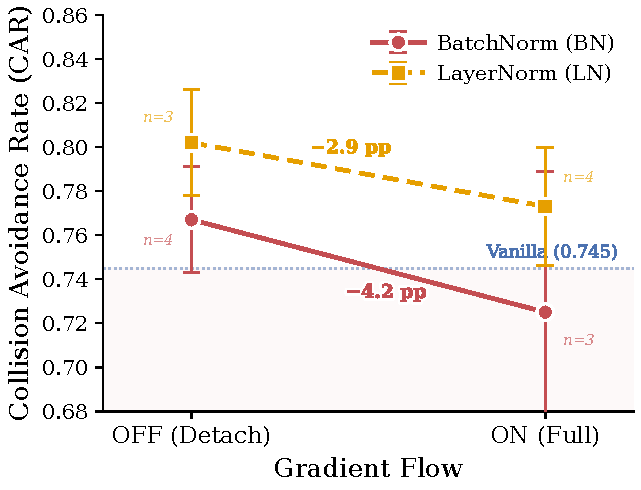
\includegraphics[width=\columnwidth]{figures/factorial_2x2_pb.pdf}
% \caption{...}
% \label{fig:factorial_old}
% \end{figure}

\begin{figure*}[t]
\centering
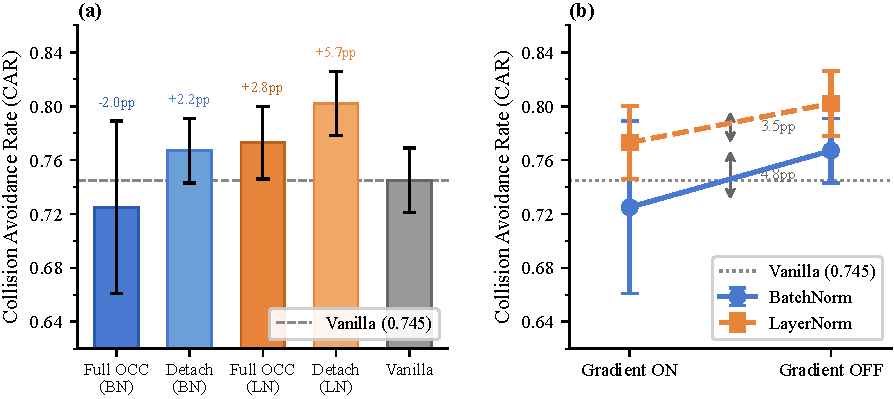
\includegraphics[width=\textwidth]{figures/fig_car_factorial_combined.pdf}
\caption{(a)~Only BN + gradient flow falls below Vanilla. Detach+LN achieves the highest CAR ($0.802{\pm}0.024$, $n{=}3$), consistently outperforming Vanilla ($0.745$; Hedges' $g{=}1.89$). Error bars: cross-seed SD. (b)~Classic interaction plot: near-parallel lines indicate negligible interaction ($p_\text{perm}{=}0.794$). LN consistently outperforms BN by 3.5--4.8\,pp regardless of gradient flow. Only BN + gradient ON falls below Vanilla.}
\label{fig:car_factorial}
\end{figure*}

\subsection{Factorial Interpretation}

\textbf{Gradient flow is associated with lower safety under BatchNorm but not under LayerNorm.} Full OCC (BN) is the sole cell below Vanilla ($\Delta{=}-2.0$\,pp), while all other cells exceed it (Table~\ref{tab:factorial}). Detach+LN yields the highest mean ($0.802$, $g{=}+1.89$; bootstrap 95\% CI for $\Delta$: $[0.025, 0.089]$). This is a practical threshold crossing rather than a statistical interaction ($\eta^2{=}0.005$).

\textbf{Temporal dynamics.} Cutoff conditions illuminate when gradient flow's association with lower safety emerges. Cutoff@15K ($\Delta{=}+0.2$\,pp) performs near Vanilla, while Cutoff@25K exhibits a deficit ($\Delta{=}-5.6$\,pp, $n{=}2$) and Cutoff@35K returns to baseline ($\Delta{=}-0.1$\,pp). Cutoff@45K ($\Delta{=}-1.6$\,pp, single seed) falls between these extremes. This non-monotonic pattern suggests that the critical window for the gradient flow safety deficit is not simply cumulative exposure but depends on the training phase. Reverse Cutoff (gradient flow only after step 35K, $n{=}2$) yields the lowest supplementary CAR ($\Delta{=}-6.2$\,pp); late-stage gradient flow, when the model is refining action predictions, is associated with substantially worse outcomes than early exposure during initial representation learning. However, temporal conditions use 1--3 seeds (v1); these observations are preliminary.

\subsection{Gradient Dynamics}

Gradient analysis (Figure~\ref{fig:gradient_analysis}) examines the mechanism through which auxiliary heads affect safety. All gradient norms are computed with respect to the L1 action loss (action tokens only).

\begin{figure*}[t]
\centering
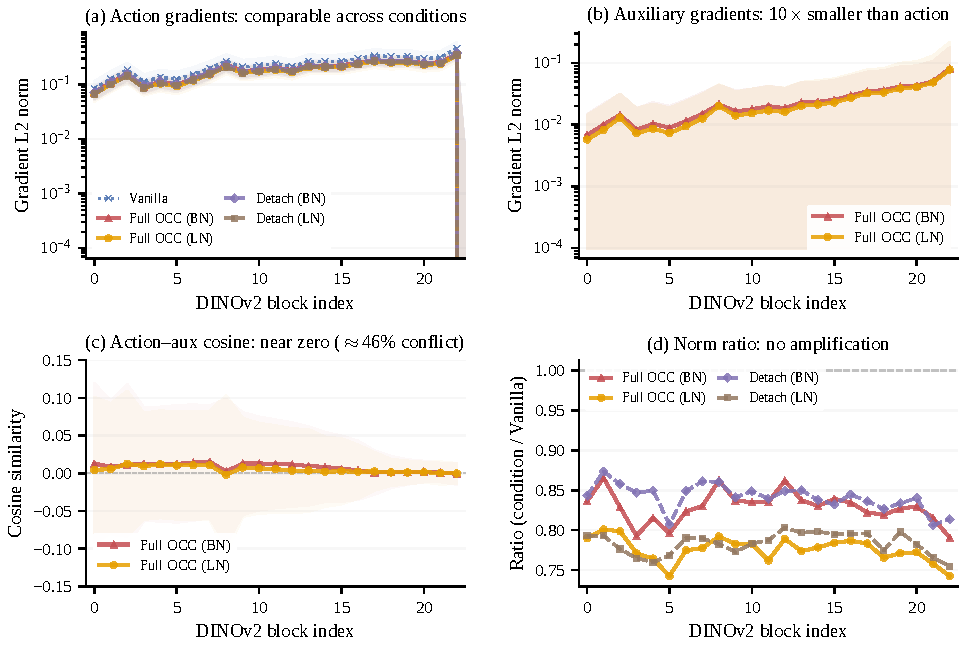
\includegraphics[width=\textwidth]{figures/gradient_analysis_v2_combined.pdf}
\caption{Gradient dynamics (v2, seed 42, 200 batches at 50K; Random OCC data obtained under v1 codebase). Action gradient norms are comparable across conditions, ruling out amplification. Action--auxiliary cosine similarity is near zero (${\approx}$46\% conflict rate), consistent with orthogonality.}
\label{fig:gradient_analysis}
\end{figure*}

\textbf{Gradient orthogonality rules out direct conflict.} Action--auxiliary gradient cosine similarity is near zero across all encoder layers for both Full OCC and Random OCC (Figure~\ref{fig:gradient_analysis}), with conflict rates of ${\approx}$46\%. Action loss gradient norms are comparable across Vanilla and gradient-flow conditions (Figure~\ref{fig:gradient_analysis}), ruling out gradient amplification. Both patterns are identical for structured and random labels, consistent with the behavioral finding that spatial content did not detectably affect outcomes. (Random OCC gradient data were obtained under the v1 codebase; the v2 gradient analysis covers all four factorial conditions and Vanilla, each using a v2-trained checkpoint.)

\textbf{Mechanism remains open.} Neither gradient conflict nor amplification explains the effect. CKA analysis~\cite{kornblith2019similarity} confirms intact encoder representations (CKA $\geq$ 0.95 across all layers), localizing the safety deficit to optimization dynamics---likely subtle LoRA adapter weight differences invisible to representational similarity measures.

Additional observations (per-task breakdown, depth comparison, and temporal dynamics) are in Appendix~\ref{app:additional}.



\section{Discussion}
\label{sec:discussion}

\textbf{Excluded mechanism: gradient conflict.} Near-zero action--auxiliary cosine similarity (${\approx}$46\% conflict rate; Figure~\ref{fig:gradient_analysis}) and comparable action gradient norms (Figure~\ref{fig:gradient_analysis}) rule out PCGrad-style gradient conflict~\cite{yu2020pcgrad}.
%
\textbf{Hypothesis: BN forward-pass statistics corruption.} BatchNorm is not inherently harmful: Detach OCC (BN, gradient OFF) matches Vanilla ($0.767$ vs.\ $0.745$, $p{=}0.28$); the deficit requires the joint presence of BN and gradient flow. We hypothesize a \emph{forward-pass} mechanism: BN running mean/variance update during each forward pass regardless of gradient conflict, so the auxiliary head shifts the running statistics used at inference. LayerNorm, normalizing per-token without cross-batch statistics, lacks this coupling. CKA confirms intact encoder representations (CKA $\geq$ 0.95), localizing the effect to optimization dynamics rather than representational corruption (a targeted test: comparing BN in train vs.\ eval mode at inference would isolate the running-statistics channel).

\textbf{Normalization independently affects safety.} LN provides a consistent $+$3.5--4.8\,pp advantage over BN ($g{=}0.88$--$1.24$). This advantage amplifies fourfold on the three physically constrained tasks ($+6.9$\,pp vs.\ $+1.7$\,pp; Appendix~\ref{app:per_task_factorial}), concentrating where safety margins are thinnest. Normalization type, typically treated as an implementation detail, has outsized consequences for safety-critical VLA fine-tuning.

\textbf{Additive effects.} Detach+LN achieves the best safety (CAR $0.802$), outperforming Vanilla ($g{=}1.89$, bootstrap 95\% CI for $\Delta$: $[0.025, 0.089]$). The advantage arises from two independent effects (${\approx}$3--5\,pp each; interaction $\eta^2{=}0.005$). Only BN + gradient flow falls below Vanilla; removing either condition restores safety. Additivity is consistent with two mechanistically distinct pathways: normalization type governs forward-pass statistics computation (a data-flow property), while gradient flow governs backward-pass parameter updates (an optimization property). If these pathways are orthogonal, independent corrections are expected---each fix helps regardless of the other's state.

\textbf{Codebase sensitivity.} A code revision (v2) shifts absolute CAR by up to 8.6\,pp, exceeding the largest experimental effect (${\leq}5.7$\,pp; Appendix~\ref{app:codebase}). Non-hyperparameter implementation details can dominate the signal of interest.

\textbf{Content irrelevance.} Structured, random, and depth labels produce indistinguishable safety outcomes (observed under the original codebase), consistent with action--auxiliary orthogonality. No ground-truth spatial annotations are required.

\textbf{Safety--success dissociation.} Full OCC (BN) maintains comparable task success (TSR $0.854$) yet exhibits the worst safety (CAR $0.725$), so standard task-success benchmarks cannot serve as safety proxies~\cite{li2026spatialforcing, yuan2025depthvla, wu2025spatialvla, liu2025occvla}. Collision avoidance demands fine-grained trajectory control near obstacles, where small perturbations cross boundaries; task success tolerates larger deviations.

\textbf{Practical guideline.} Use detached gradients with LayerNorm; the head is discarded at inference (zero overhead). Loss weighting~\cite{kendall2018uncertainty} does not address the forward-pass BN mechanism. Given codebase sensitivity, guidelines should be verified per implementation.

\textbf{Generalizability.} Normalization type and gradient flow are architectural choices common to all auxiliary-head VLA pipelines. The BN running-statistics mechanism is not architecture-specific; we expect the qualitative pattern to transfer, though effect sizes may vary.



\section{Conclusion}

We presented the first factorial study of auxiliary spatial supervision during VLA fine-tuning. Detached gradients with LayerNorm consistently outperforms the no-auxiliary baseline, while BatchNorm with gradient flow reduces safety below it. The two effects combine additively, with the normalization advantage amplifying fourfold on physically constrained tasks. The content of spatial labels has no detectable effect---the critical factor is not \emph{what} the auxiliary head predicts but \emph{how} it interacts with the shared encoder during training. The safety deficit is not accompanied by task-success degradation (TSR ANOVA all $p{>}0.27$). Three zero-cost guidelines follow: detach gradients under BN; prefer LN; ground-truth labels are unnecessary. Future work should verify the BN hypothesis, extend to other architectures and benchmarks, and integrate with runtime safety methods.



\section{Limitations}

\textbf{Simulation only.} All experiments use simulated tabletop tasks; real-robot transfer is untested. Real-world contact dynamics, sensor noise, and control latency introduce failure modes absent in simulation that may alter the relative safety ranking. Validating on physical hardware is a necessary next step.
%
\textbf{Single model and benchmark.} We study one architecture (OpenVLA-7B with LoRA) on one benchmark (SafeLIBERO Level~I). The factorial effects may differ for other VLA families, model scales, or collision definitions. Architectures with different normalization defaults (e.g., $\pi_0$ with GroupNorm, Octo with LayerNorm) may exhibit different sensitivity profiles. Extending to additional architectures would strengthen generalizability.
%
\textbf{Codebase sensitivity.} A code revision shifted CAR by up to 8.6\,pp, exceeding the largest experimental effect; conclusions may not transfer across codebases without re-verification.
%
\textbf{Unverified mechanism.} The BN running-statistics hypothesis is mechanistically plausible but not directly tested; a targeted BN eval-mode ablation would isolate this channel. All conditions use LoRA; effects under full fine-tuning are untested. Content ablations were conducted under the original codebase only.


\bibliography{references}

\clearpage
\appendix

\section{Extended Per-Task Results}
\label{app:per_task}

Table~\ref{tab:per_task} reports per-task mean CAR across seeds for each condition. Seven tasks achieve CAR $\geq$ 0.92 under Vanilla, while three physically constrained tasks (T3, T5, T6) fall below 0.58. The overall CAR differences reported in the main text are dominated by these three hard tasks, which average 0.342 compared to 0.968 for the seven non-hard tasks.

\begin{table}[h]
\centering
\caption{Per-task mean CAR across seeds (50 rollouts per seed, v1 code). This table reports v1 codebase results retained for completeness; all main analyses use v2 data (Table~\ref{tab:main_results}). All conditions use 3 seeds except Depth (4). Detach+LN per-task uses 2 seeds (s1, s2; s0 lacks per-task breakdown).}
\label{tab:per_task}
\begin{tabular}{clccccccc}
\toprule
 & & \multicolumn{7}{c}{Mean CAR by Condition} \\
\cmidrule(lr){3-9}
Task & Diff. & Vanilla & Full OCC & Random & Detach & Det+LN & Depth & Cut@35K \\
\midrule
T0 & Easy  & 0.98 & 0.98 & 0.99 & 0.97 & 0.97 & 0.99 & 0.98 \\
T1 & Easy  & 0.92 & 0.93 & 0.99 & 0.89 & 0.78 & 0.93 & 0.95 \\
T2 & Easy  & 0.92 & 0.93 & 0.94 & 0.93 & 0.90 & 0.90 & 0.94 \\
T3 & Hard  & 0.38 & 0.37 & 0.31 & \textbf{0.11} & 0.44 & 0.50 & 0.55 \\
T4 & Med   & 0.98 & 0.99 & 0.95 & 0.98 & 0.96 & 0.92 & 0.97 \\
T5 & Hard  & 0.07 & 0.17 & 0.23 & \textbf{0.05} & 0.12 & 0.08 & 0.04 \\
T6 & Hard  & 0.57 & 0.61 & 0.55 & 0.56 & 0.36 & 0.54 & 0.38 \\
T7 & Easy  & 0.97 & 0.99 & 0.95 & 0.98 & 1.00 & 0.96 & 0.98 \\
T8 & Easy  & 1.00 & 1.00 & 1.00 & 0.99 & 0.99 & 0.99 & 0.99 \\
T9 & Easy  & 1.00 & 0.99 & 0.99 & 1.00 & 1.00 & 1.00 & 1.00 \\
\midrule
\multicolumn{2}{l}{Overall} & 0.780 & 0.797 & 0.789 & 0.746 & 0.765 & 0.780 & 0.779 \\
\bottomrule
\end{tabular}
\end{table}

\textbf{Ceiling effects.} On the seven non-hard tasks (T0--T2, T4, T7--T9), most conditions achieve CAR $\geq$ 0.89, with isolated exceptions (e.g., Detach+LN T1 ${=}$ 0.78), leaving minimal room for auxiliary training to improve performance. The obstacle is spatially separated from the manipulation path in these tasks.

\textbf{Hard task patterns.} On Task~5 (Vanilla CAR 0.07), gradient-flow conditions (Random OCC 0.23, Full OCC 0.17) exceed Vanilla and Detach (0.05), but all values remain below 0.23. Cutoff@35K achieves the highest T3 CAR (0.55) but the lowest T5 CAR (0.04), which illustrates task-specific temporal sensitivity. Depth exhibits high cross-seed variance on hard tasks (T3 range: 0.20--0.78; T6 range: 0.16--0.84), consistent with auxiliary supervision increasing seed sensitivity.

\section{Training Details}
\label{app:training}

\begin{table}[h]
\centering
\caption{Training hyperparameters.}
\begin{tabular}{ll}
\toprule
Parameter & Value \\
\midrule
Base model & OpenVLA-7B~\cite{kim2024openvla} \\
Fine-tuning recipe & OFT~\cite{kim2025oft} \\
Vision encoders & DINOv2 (1024-d) + SigLIP (1152-d) \\
Patch token dim. & 2176 (concatenated) \\
LoRA rank / $\alpha$ & 32 / 16 \\
LoRA trainable params & 110.8M (1.45\% of 7.65B) \\
Optimizer & AdamW (weight decay 0.01) \\
Batch size & 8 \\
Learning rate & $5 \times 10^{-4}$ (constant) \\
Training steps & 50{,}000 \\
Aux.\ loss weight $\lambda_0$ & 0.01 \\
Aux.\ loss decay & $\exp(-t / 50{,}000)$ \\
BEV grid resolution & $64 \times 64$ \\
Focal loss $\alpha$ / $\gamma$ & 0.25 / 2.0 \\
Depth loss & Smooth-L1 \\
Aux.\ head parameters & 1.2M \\
Hardware & NVIDIA RTX PRO 6000 (96\,GB) \\
Wall time per run & $\sim$12.9 hours \\
\bottomrule
\end{tabular}
\end{table}

\textbf{Evaluation protocol.} Each condition uses 3+ seeds (Depth uses 4; Cutoff@15K, Cutoff@25K, and Reverse Cutoff use 2; Cutoff@45K uses 1) with 50 rollouts per task per seed (500 episodes per seed). A collision is registered when the L1 displacement of the obstacle's \texttt{body\_xpos} exceeds $10^{-3}$. Bootstrap 95\% CIs are computed via 10{,}000 resamples (percentile method).

\textbf{Statistical tests.} Pairwise comparisons against Vanilla use two-tailed permutation tests on per-seed mean CARs with Hedges' $g$ (bias-corrected for small samples) for effect size. With $n{=}3$ seeds, statistical power is limited; we report $p$-values and effect sizes for transparency.
\textbf{CKA analysis.} Centered Kernel Alignment~\cite{kornblith2019similarity} measures representational similarity between fine-tuned and pretrained encoder features. We extract patch token activations from the final layer of DINOv2 and SigLIP for 1{,}000 validation images, compute linear CKA per layer, and report the mean across layers. Higher CKA indicates better preservation of pretrained representations.

\textbf{Cutoff implementation.} As described in Section~\ref{sec:ablation}, setting $\lambda(t){=}0$ does not disable the auxiliary head's forward pass; the post-cutoff phase operates in Detach mode with BatchNorm statistics continuing to update (see the Cutoff description therein for details).

\section{Extended Analysis}

% Figure~\ref{fig:gradient_analysis} is in the main text (Results, Gradient Dynamics subsection).

The Detach+LN ablation replaces BatchNorm2d with LayerNorm in the auxiliary head while retaining \texttt{stop\_gradient}. Under v1 (3 seeds), Detach+LN achieves CAR $0.765 \pm 0.023$; under v2 ($n{=}3$), Detach+LN achieves $0.802 \pm 0.024$ (Table~\ref{tab:main_results}), the highest factorial cell mean ($\Delta{=}+5.7$\,pp vs.\ Vanilla, $g{=}+1.89$). This confirms the additive main effects: both detaching gradient flow and using LN independently improve safety.

\textbf{Per-layer gradient analysis.} Figure~\ref{fig:per_layer_combined} decomposes auxiliary gradient flow into two dimensions: amplitude (top row) and direction (bottom row). The amplitude heatmap (panels a--b) shows that Vanilla, Full OCC, and Random OCC maintain comparable action gradient norms across all layers (warm colors), while Detach shows substantially reduced norms across both encoders (dark). These amplitude results were generated from v1 codebase checkpoints. The v2 gradient analysis (Figure~\ref{fig:gradient_analysis}) confirms that the Detach gradient suppression does not reproduce: Detach and gradient-flow conditions maintain comparable action gradient norms under v2, indicating the v1 suppression was a code-path artifact (see Appendix~\ref{app:codebase}). The directional analysis (panels c--d) reveals encoder-specific alignment: DINOv2 conflict rates hover near 46\% across all layers while SigLIP late layers (blocks 21--24) drop to 19--25\%, which indicates cooperative gradient alignment in semantically rich layers. Both patterns are identical for Full OCC and Random OCC, which confirms they arise from architectural structure rather than label content. The aggregate conflict rates (Full OCC 45.6\%, Full OCC+LN 45.7\% under v2; Full OCC 44.1\%, Random OCC 43.9\% under v1) fall below the 50\% expected for random vectors because they reflect this mixture of two encoder-specific patterns.

\begin{figure}[h]
\centering
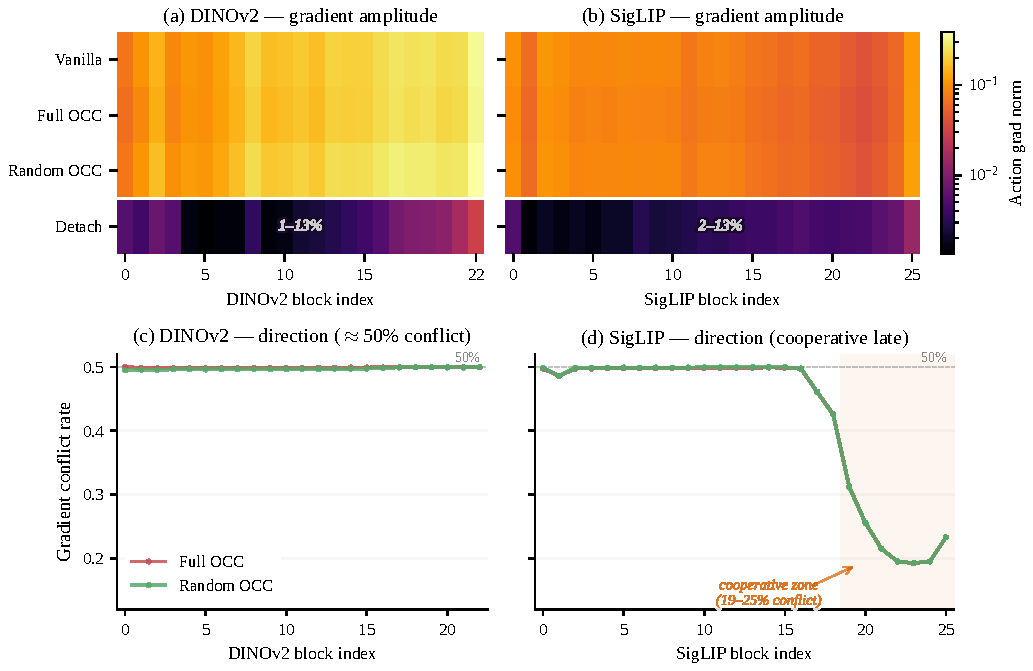
\includegraphics[width=\textwidth]{figures/per_layer_combined.pdf}
\caption{Per-layer gradient analysis decomposed into amplitude and direction (v1 codebase checkpoint, seed 42, 200 batches). \textbf{Top (a--b):} Action gradient norm heatmap (log scale). Gradient-flow conditions (Vanilla, Full OCC, Random OCC) maintain comparable norms; Detach shows substantially reduced norms across all layers, a v1-specific artifact not reproduced under v2 (see Appendix~\ref{app:codebase}). \textbf{Bottom (c--d):} Gradient conflict rate between action and auxiliary losses. DINOv2 maintains $\sim$46\% conflict (near-orthogonal), while SigLIP late layers drop to 19--25\% (cooperative alignment). Both amplitude and directional patterns are identical for Full OCC and Random OCC, confirming architectural rather than label-dependent structure. Directional findings are confirmed under v2; the Detach amplitude suppression (a--b) is a v1 code-path artifact. Conflict rates approach ${\approx}$46\% in early and middle layers; late SigLIP layers show lower conflict rates (${\approx}$25\%), consistent with weak alignment rather than conflict.}
\label{fig:per_layer_combined}
\end{figure}

\subsection{Temporal Dynamics}
\label{app:temporal}
\textbf{Dose-response: gradient flow duration vs.\ CAR (v1 data).} Figure~\ref{fig:dose_response} plots CAR against the number of OCC gradient flow steps for the cutoff series (15K--45K, plus Detach at 0K and Full OCC at 50K; all v1 code). Cutoff@15K (2 seeds, CAR 0.782) clusters near Vanilla (0.780), while Cutoff@25K (2 seeds, 0.724) falls substantially below. Multi-seed conditions (Cutoff@35K and Full OCC) also cluster near the Vanilla baseline. Reverse Cutoff (late 15K) falls below the early-cutoff counterpart at the same gradient flow duration, consistent with the continuity hypothesis. The pattern suggests intermediate cutoff $\approx$ Vanilla rather than a non-monotonic dose-response; the earlier single-seed Cutoff@15K result (0.804) was seed noise.

\begin{figure}[h]
\centering
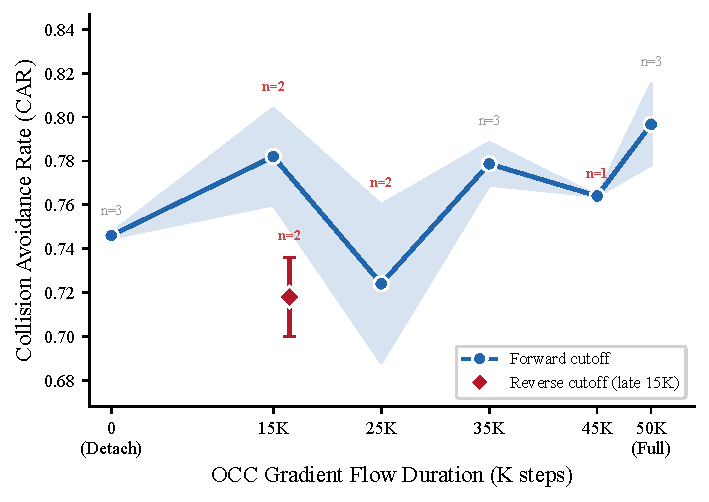
\includegraphics[width=0.75\textwidth]{figures/dose_response.pdf}
\caption{Dose-response: CAR vs.\ OCC gradient flow duration (v1 codebase, all conditions). Filled circles: early-cutoff conditions with all 3 seeds completed; open circles: conditions with $\leq$2 seeds (counts annotated as $n$). Diamond ($\diamond$): Reverse Cutoff (gradient flow restricted to the last 15K steps). Dashed line: Vanilla 3-seed mean (v1); shaded band: $\pm\,$1\,SE. The ``+0.2\%'' annotation marks the Cutoff@15K--Vanilla gap. Intermediate cutoff conditions cluster near Vanilla, while Cutoff@25K and Reverse Cutoff fall substantially below.}
\label{fig:dose_response}
\end{figure}

\section{Additional Observations}
\label{app:additional}

\textbf{Per-task concentration.} Seven of ten tasks achieve CAR $\geq$ 0.92 under Vanilla; overall CAR is dominated by three physically constrained tasks (T3, T5, T6; Section~\ref{app:per_task}). Under the v1 codebase, Detach showed the lowest CAR on these hard tasks (T3: 0.11, T5: 0.05). However, this v1-specific pattern does not replicate under the controlled v2 factorial design (Table~\ref{tab:main_results}), where detaching gradient flow consistently preserves safety (Detach OCC CAR 0.767 vs.\ Vanilla 0.745); the v1 per-task pattern may reflect implementation-specific artifacts rather than a generalizable effect of gradient detachment.

\textbf{Egocentric depth matches Vanilla (v1 data).} Depth (4 seeds) achieves CAR 0.780 $\pm$ 0.039, identical to Vanilla (v1, 0.780), despite providing per-pixel geometric information. Three label types (structured BEV, random binary, egocentric depth) yield comparable CAR when gradient flow is maintained.

\textbf{Temporal dynamics (preliminary, v1 data).} Cutoff@35K (3 seeds) achieves CAR 0.779, statistically indistinguishable from Vanilla (v1, $\Delta = -$0.1\,pp), which confirms that 35K steps of gradient flow fully protects collision avoidance. Surprisingly, Cutoff@25K (0.724, 2 seeds) and Reverse Cutoff (0.718, 2 seeds) fall substantially \emph{below} Vanilla. The most parsimonious explanation: setting the loss weight to zero retains the auxiliary head forward pass, so the post-cutoff period operates in Detach mode; BatchNorm interference acts on representations shaped by gradient flow, without gradient compensation. This is not withdrawal from gradient flow \emph{per se}, but transition into a regime associated with lower safety. Third seeds are in progress; extended analysis in Section~\ref{app:temporal}.

\section{Codebase Sensitivity (v1 vs.\ v2)}
\label{app:codebase}

The five core factorial conditions were retrained under a revised codebase (v2) that fixed a batch-index resume bug affecting cutoff timing and restructured the auxiliary head pipeline (module initialization order, data loading). All model architectures, hyperparameters, LoRA configuration, and evaluation protocols are identical between v1 and v2. The Vanilla baseline (no auxiliary head) is unaffected by these changes, since the revision touches only auxiliary-head code paths.

\textbf{Behavioral shift.} Under v1, Full OCC achieved a mean CAR of 0.797 (3 seeds, per-task Table~\ref{tab:per_task}); under v2, the same condition yields 0.725 $\pm$ 0.064 (Table~\ref{tab:main_results}). Same-seed comparisons show shifts of up to 8.6\,pp, while Vanilla remains stable across codebases ($<$1.5\,pp). This sensitivity is confined to conditions with auxiliary heads and is itself informative: it indicates that auxiliary head training dynamics are fragile with respect to implementation details that would not normally be considered hyperparameters.

\textbf{Gradient analysis shift.} The v1 codebase exhibited a Detach gradient suppression artifact: Detach action-loss gradient norms were only $\sim$4\% of Vanilla norms across all encoder layers. In v2, this suppression disappears entirely (Detach/Vanilla ratio $\approx$ 1.29), indicating that the v1 pattern was a code-path artifact rather than a genuine effect of gradient detachment. The gradient conflict rate also shifted from $\sim$44\% (v1) to $\sim$46\% (v2), with v2 values closer to the theoretical expectation for orthogonal vectors.

\textbf{Effect pattern shift.} Under v1, the normalization $\times$ gradient flow pattern appeared as a crossover ($p{=}0.025$); under v2, both rows slope in the same direction, consistent with two additive main effects rather than an interaction (ANOVA interaction $F{=}0.10$, $p{=}0.763$, $\eta^2{=}0.005$). The crossover pattern in v1 is likely attributable to the Detach gradient suppression artifact described above, which differentially affected BN and LN conditions. All main-text analyses use v2 data exclusively; v1 results are retained in the appendix for completeness and to document the sensitivity.

\textbf{Implication.} The codebase sensitivity reinforces our central finding: auxiliary spatial heads introduce optimization fragility that implementation details can amplify or attenuate. This fragility is a further argument against adding auxiliary spatial heads for safety purposes, since the safety outcome depends on implementation choices that are difficult to specify, reproduce, or audit.

\section{Statistical Power Analysis}
\label{app:stat_power}

The $2{\times}2$ factorial design prioritizes breadth (12 conditions, 5 factors) over per-cell statistical power. With $n{=}3$--$4$ per cell (14 total observations), the design yields medium power for the observed effect sizes. The normalization main effect approaches significance ($p{=}0.060$, $\eta^2{=}0.253$); the gradient flow main effect does not reach significance ($p{=}0.104$) but shows a medium-to-large effect size ($\eta^2{=}0.180$). We report effect sizes as the primary inferential quantity.

The study's evidential strength rests on the consistent direction of both main effects: both BN and LN rows show lower CAR under gradient flow ON than OFF, and both gradient flow conditions show higher CAR under LN than BN. The negligible interaction ($\eta^2{=}0.005$) confirms these effects are additive.

\textbf{Formal $2{\times}2$ ANOVA.} Table~\ref{tab:anova} reports the Type~II factorial analysis ($n{=}3$--$4$ per cell, 14 total observations). The interaction is negligible ($F(1,10){=}0.10$, $p{=}0.763$, $\eta^2{=}0.005$), confirming additive main effects. The normalization main effect approaches significance ($F(1,10){=}4.49$, $p{=}0.060$, $\eta^2{=}0.253$); the gradient flow main effect is medium-sized but non-significant ($F(1,10){=}3.20$, $p{=}0.104$, $\eta^2{=}0.180$). The non-significant gradient flow $p$-value reflects limited per-cell power rather than an absent effect.

\begin{table}[h]
\centering
\caption{$2{\times}2$ factorial ANOVA (Type~II SS). The interaction is negligible; the normalization main effect approaches significance ($p{=}0.060$).}
\label{tab:anova}
\begin{tabular}{lcccc}
\toprule
Source & $F$ & df & $p$ & $\eta^2$ \\
\midrule
Gradient flow (ON vs.\ OFF) & 3.20 & 1,\,10 & 0.104 & 0.180 \\
Normalization (BN vs.\ LN) & 4.49 & 1,\,10 & 0.060 & 0.253 \\
Interaction & 0.10 & 1,\,10 & 0.763 & 0.005 \\
\bottomrule
\end{tabular}
\end{table}

\textbf{Pairwise effect sizes.} Table~\ref{tab:pairwise} reports Hedges' $g$ (bias-corrected) for all factorial cell pairs and versus Vanilla ($n{=}3$--$4$ per cell).

\begin{table}[h]
\centering
\caption{Pairwise Hedges' $g$ (bias-corrected) for factorial cells and Vanilla.}
\label{tab:pairwise}
\small
\begin{tabular}{lc}
\toprule
Comparison & Hedges' $g$ \\
\midrule
Cell~1 (Full OCC BN) vs.\ Cell~2 (Full OCC+LN) & $-$0.88 \\
Cell~1 vs.\ Cell~3 (Detach OCC) & $-$0.78 \\
Cell~1 vs.\ Cell~4 (Detach+LN) & $-$1.28 \\
Cell~2 vs.\ Cell~3 & $+$0.22 \\
Cell~2 vs.\ Cell~4 & $-$0.94 \\
Cell~3 vs.\ Cell~4 & $-$1.24 \\
\addlinespace
Cell~1 vs.\ Vanilla & $-$0.34 \\
Cell~2 vs.\ Vanilla & $+$0.90 \\
Cell~3 vs.\ Vanilla & $+$0.74 \\
Cell~4 vs.\ Vanilla & $+$1.89 \\
\bottomrule
\end{tabular}
\end{table}

\section{Permutation-Based ANOVA}
\label{app:permutation}

To complement the parametric $F$-test (Table~\ref{tab:anova}), we conduct a permutation-based ANOVA~\cite{anderson2001permanova} that makes no distributional assumptions. Following standard practice for factorial designs~\cite{montgomery2017doe}, we use the Type~II $F$-statistic as the test statistic and permute the 14 per-seed CAR values across all cells (10{,}000 permutations). The permutation $p$-value is the proportion of permuted $F$-statistics $\geq$ the observed value.

\begin{table}[h]
\centering
\caption{Permutation-based ANOVA for the $2{\times}2$ factorial (10{,}000 permutations). Both main effects are significant or near-significant; the interaction remains negligible.}
\label{tab:permanova}
\begin{tabular}{lccc}
\toprule
Source & $p_\text{parametric}$ & $p_\text{perm}$ & $\eta^2$ \\
\midrule
Gradient flow (ON vs.\ OFF) & 0.104 & 0.090 & 0.180 \\
Normalization (BN vs.\ LN) & 0.060 & 0.041 & 0.253 \\
Interaction & 0.763 & 0.794 & 0.005 \\
\bottomrule
\end{tabular}
\end{table}

The permutation test yields stronger evidence for the normalization main effect ($p_\text{perm}{=}0.041$, significant at $\alpha{=}0.05$) than the parametric $F$-test ($p{=}0.060$), consistent with the parametric test being conservative for small, non-normal samples. The gradient flow effect does not reach significance under permutation ($p_\text{perm}{=}0.090$) but retains a large effect size ($\eta^2{=}0.180$). The interaction remains negligible ($p_\text{perm}{=}0.794$), confirming the additive pattern.

\textbf{Bayesian model comparison.} A BIC-based Bayes Factor~\cite{wagenmakers2007practical} compares the additive model (main effects only) against a model including the interaction term: $\text{BF}_{01}{=}3.5$, providing moderate evidence that the additive model is preferred. The data are $3.5{\times}$ more likely under the no-interaction model, consistent with the negligible frequentist interaction ($\eta^2{=}0.005$).

\textbf{Safety specificity (TSR).} Applying the same $2{\times}2$ ANOVA to Task Success Rate yields no significant effects (gradient $F(1,10){=}0.85$, $p{=}0.380$; normalization $F(1,10){=}1.34$, $p{=}0.274$; interaction $F(1,10){=}1.08$, $p{=}0.322$), confirming that the safety deficit is specific to collision avoidance and does not reflect general task performance degradation.

\textbf{Leave-one-out sensitivity.} Removing each of the 14 observations and recomputing the ANOVA confirms that both effect directions are robust: $F_\text{gradient} \in [1.73, 6.05]$ (always ON ${<}$ OFF) and $F_\text{norm} \in [3.06, 7.91]$ (always BN ${<}$ LN) across all 14 deletions. The Cell~1 outlier ($\text{CAR}{=}0.654$) inflates but does not create the gradient effect (removing it: $F{=}1.73$, direction preserved); removing the highest Cell~1 seed ($0.776$) strengthens both effects to significance ($p_\text{gradient}{=}0.036$, $p_\text{norm}{=}0.020$), indicating that the reported effects are conservative.

\textbf{Variance heterogeneity.} Levene's test (Brown--Forsythe) does not reject variance homogeneity ($W{=}0.71$, $p{=}0.57$), though the test has limited power at these sample sizes ($n{=}3$--$4$ per cell) and Cell~1 exhibits $5$--$7{\times}$ the variance of other cells ($\sigma^2{=}0.0041$ vs.\ $0.0006$--$0.0007$ for other cells). Welch-corrected marginal tests yield $p{=}0.204$ (gradient) and $p{=}0.104$ (normalization); the attenuation relative to the permutation ANOVA reflects Cell~1's inflated variance entering the standard error. Both effect directions remain consistent under all corrections.

\section{Per-Task Factorial Analysis}
\label{app:per_task_factorial}

The three physically constrained tasks (T3: \texttt{cookie\_box}, T5: \texttt{ramekin}, T6: \texttt{next\_to\_cookie\_box}) show disproportionately large normalization effects under the v2 factorial design.

\textbf{Normalization effect amplification.} The LN advantage over BN averages $+6.9$\,pp on constrained tasks versus $+1.7$\,pp on easy tasks, an approximately $4{\times}$ amplification. All three constrained tasks show positive LN$-$BN differences: T6 ($+9.0$\,pp), T5 ($+7.7$\,pp), T3 ($+4.0$\,pp). The gradient flow effect, by contrast, does not concentrate on constrained tasks ($-1.6$\,pp hard vs.\ $-3.0$\,pp easy), indicating that the two effects have distinct per-task profiles.

\textbf{Cell~1 instability on constrained tasks.} Cell~1 (BN + gradient ON) exhibits $2.4{\times}$ higher cross-seed standard deviation on constrained tasks (mean $\sigma{=}0.217$) than on easy tasks ($\sigma{=}0.092$), consistent with the BN instability mechanism being most consequential where safety margins are thinnest.

\begin{table}[h]
\centering
\caption{Per-task normalization effect by task difficulty (v2 data, seed-weighted means). The LN advantage amplifies ${\approx}4{\times}$ on physically constrained tasks. T4 excluded (medium difficulty).}
\label{tab:per_task_norm}
\small
\begin{tabular}{lccc}
\toprule
Task Group & BN & LN & $\Delta$(LN$-$BN) \\
\midrule
Hard (T3, T5, T6) & $0.288$ & $0.357$ & $+6.9$\,pp \\
Easy (T0--T2, T7--T9) & $0.945$ & $0.962$ & $+1.7$\,pp \\
\bottomrule
\end{tabular}
\end{table}

% Limitations moved to main text


\end{document}
